\documentclass[12pt]{article}

% UTF-8 encoding and fonts
\usepackage[utf8]{inputenc}
\usepackage[T1]{fontenc}
\usepackage{lmodern}

% Page setup
\usepackage[margin=1in]{geometry}
\usepackage{setspace}
\onehalfspacing

% Typography
\usepackage{microtype}

% Math and symbols
\usepackage{amsmath,amssymb}

% Graphics
\usepackage{graphicx}
\usepackage{float}
\usepackage{subcaption}

% Tables
\usepackage{booktabs}
\usepackage{array}
\usepackage{multirow}
\usepackage{threeparttable}
\usepackage{longtable}
\usepackage{pdflscape}
\usepackage{siunitx}
\usepackage{adjustbox}
\sisetup{detect-all=true, group-separator={,}, group-minimum-digits=4}

% Bibliography
\usepackage{natbib}
\bibliographystyle{aer}

% Hyperlinks
\usepackage{hyperref}
\hypersetup{
    colorlinks=true,
    linkcolor=blue,
    citecolor=blue,
    urlcolor=blue
}
\usepackage[nameinlink,noabbrev]{cleveref}

% Timing data
\IfFileExists{timing_data.tex}{\input{timing_data.tex}}{
  \newcommand{\apepcurrenttime}{N/A}
  \newcommand{\apepcumulativetime}{N/A}
}

% Captions
\usepackage{caption}
\captionsetup{font=small,labelfont=bf}

% Section formatting
\usepackage{titlesec}
\titleformat{\section}{\large\bfseries}{\thesection.}{0.5em}{}
\titleformat{\subsection}{\normalsize\bfseries}{\thesubsection}{0.5em}{}

% Custom commands
\newcommand{\E}{\mathbb{E}}
\newcommand{\Var}{\text{Var}}
\newcommand{\Cov}{\text{Cov}}
\newcommand{\ind}{\mathbb{I}}
\newcommand{\sym}[1]{\ifmmode^{#1}\else\(^{#1}\)\fi}

\title{The Price of a National Pay Scale: Teacher Competitiveness and Student Value-Added in England\footnote{This paper is a revision of apep\_0483. See \url{https://github.com/SocialCatalystLab/ape-papers/tree/main/apep_0483} for the original.}}
\author{APEP Autonomous Research\thanks{Autonomous Policy Evaluation Project. Correspondence: scl@econ.uzh.ch{} (cumulative: \apepcumulativetime{}).} \and @SocialCatalystLab}
\date{\today}

\begin{document}

\maketitle

\begin{abstract}
\noindent
In 2010, England's teachers earned a third more than local private-sector workers. By 2023, surging private wages had eroded that premium to 27\%. We construct the first local-authority panel of teacher pay competitiveness---the ratio of teacher to private-sector earnings---and estimate its relationship with Progress~8, a value-added measure of student achievement. Within-LA fixed effects estimates are small and insignificant ($\hat{\beta} = 0.025$, SE $= 0.068$), but baseline exposure interactions reveal growing negative coefficients after the pay restraint period ($p = 0.033$). A Bartik IV yields a larger positive estimate ($\hat{\beta}_{\text{IV}} = 1.245$, $F = 14.5$), though a falsification test suggests the exclusion restriction is violated. Results are robust to region$\times$year fixed effects and excluding London. The evidence suggests competitiveness operates through slow-moving channels, but we cannot definitively establish causality.
\end{abstract}

\vspace{1em}
\noindent\textbf{JEL Codes:} I21, J31, J45, H75 \\
\noindent\textbf{Keywords:} teacher pay, competitiveness, Progress 8, value-added, austerity, England

\newpage

%=============================================================================
\section{Introduction}
%=============================================================================

In 2010, the average English teacher earned a third more than her local private-sector counterpart. By 2023, that premium had shrunk to 27\%---not because teachers took pay cuts, but because private-sector wages surged while nationally set teacher salaries barely kept pace. The erosion was not uniform: in London and the South East, where private-sector wages grew fastest, the teacher premium was already thin and fell further; in the North, where wages grew slowly, teaching remained relatively well-compensated.

This paper asks whether this differential erosion of teacher pay competitiveness affected student achievement. The question matters because teacher quality is the most important school-level determinant of student outcomes \citep{rivkin2005teachers, chetty2014measuring1, chetty2014measuring2}, and standard models predict that labor supply responds to relative wages \citep{hanushek2011economic}. If competitive private-sector pay draws potential teachers into other careers---or pushes incumbent teachers out of the profession---students in affected areas should suffer. The magnitude of any such effect has direct implications for the ongoing policy debate about England's teacher recruitment crisis \citep{strb2023report}.

We construct the first panel measure of teacher pay competitiveness at the local authority (LA) level, defined as the ratio of the STPCD main-scale midpoint to median annual private-sector earnings (from the Annual Survey of Hours and Earnings). Higher values indicate that teacher pay is more competitive with the private sector. This ratio varies across LAs and over time because private-sector wages are locally determined while STPCD scales---which set pay for all maintained schools---are nationally negotiated with only four geographic bands (Inner London, Outer London, Fringe, and Rest of England). As private-sector wages diverge across local labor markets, teachers face very different outside options depending on where they work.

Our identification strategy exploits within-LA variation in competitiveness over time. We estimate panel fixed effects models with LA and year fixed effects, using 157 LAs observed over 4 academic years (2018/19 and 2021/22--2023/24, excluding COVID-disrupted years). The outcome is Progress~8, England's official value-added measure, which adjusts raw exam scores for students' prior attainment at age 11 and is therefore less susceptible to compositional confounding than raw achievement measures.

Our main finding is a precisely estimated null. The within-LA estimate of the effect of competitiveness on Progress~8 is $\hat{\beta} = 0.025$ (SE $= 0.068$, $p = 0.713$). This null absorbs both time-invariant LA characteristics and common year shocks. However, the null masks important dynamics: an event study interacting baseline (2018) competitiveness with year indicators reveals growing negative coefficients for 2021/22 through 2023/24, with the 2023/24 coefficient reaching $-0.204$ ($p = 0.003$). These post-2021 coefficients are jointly significant ($p = 0.033$), suggesting that the damage from eroding competitiveness accumulates over time rather than operating contemporaneously.

To probe whether endogenous local wage growth biases our estimates, we instrument competitiveness using a Bartik-style strategy \citep{goldsmith2020bartik}, interacting 2010 baseline high-wage industry employment shares with a linear time trend. The IV estimate ($\hat{\beta}_{\text{IV}} = 1.245$, $p = 0.045$, first-stage $F = 14.5$) is positive and substantially larger than OLS. However, a falsification test reveals that the instrument also predicts Attainment~8 (raw scores unadjusted for prior attainment), raising concerns about the exclusion restriction. We interpret the IV as providing a sign check---higher competitiveness is associated with better outcomes---but caution against relying on its magnitude.

We probe mechanisms through two channels. First, we test whether competitiveness affects teacher vacancy rates using School Workforce Census data. The point estimate suggests that less competitive LAs have more vacancies, though the relationship is not precisely estimated in our sample. Second, we exploit the institutional feature that academies---which constitute 75\% of English secondary schools---can legally set their own pay outside the STPCD framework, while maintained schools cannot. If the STPCD constraint is the binding mechanism, we would expect maintained schools to show stronger effects. The academy triple-difference reveals maintained-school effects that are directionally consistent ($-0.451$) but not statistically distinguishable from the academy effect ($-0.695$, interaction $p = 0.43$). This is consistent with evidence from \citet{britton2016teacher} that most academies follow STPCD pay in practice.

Cross-sectional analysis reveals a steep gradient by deprivation: school-level Progress~8 varies strongly with LA-level competitiveness in the most deprived quartile ($\beta = -1.726$) but not in less deprived areas. We interpret this gradient cautiously: because the competitiveness ratio varies only at the LA level, cross-sectional regressions cannot include LA fixed effects and are confounded by the well-documented north--south gradient in English education. The pattern is consistent with a model in which deprived schools are most vulnerable to wage competition, but we cannot rule out confounding from unobserved LA characteristics.

While previous work on teacher pay and outcomes has relied on cross-sectional variation or studied specific pay interventions \citep{britton2016teacher, dolton2011if, hendricks2014relative, hoxby1996teachers}, we exploit a decade of nationally imposed pay restraint interacting with heterogeneous local labor markets to construct the first panel measure of teacher competitiveness across English LAs. This allows within-LA comparisons that absorb the north--south gradient confounding earlier estimates \citep{sims2020teacher, allen2018understanding, burgess2019teacher}. Our approach speaks to the broader question of how public-sector pay rigidities affect service quality \citep{clotfelter2008would}---a question with implications for any profession where pay is centrally determined but labor markets are local.

The rest of the paper proceeds as follows. Section~2 describes the institutional setting. Section~3 presents the data and measurement strategy. Section~4 describes the empirical approach. Section~5 presents results. Section~6 discusses mechanisms. Section~7 reports robustness checks. Section~8 concludes.


%=============================================================================
\section{Institutional Background}
%=============================================================================

\subsection{The STPCD and Teacher Pay in England}

Teacher pay in England's state-maintained schools is governed by the School Teachers' Pay and Conditions Document (STPCD), a statutory instrument issued annually by the Secretary of State for Education following recommendations from the School Teachers' Review Body (STRB). The STPCD sets minimum and maximum salaries for the main pay range (M1--M6), the upper pay range (UPS1--UPS3), and the leadership pay range. Schools have some discretion in where to place teachers within these ranges, but the ranges themselves are nationally determined \citep{strb2023report}.

The STPCD defines four geographic pay bands: Inner London, Outer London, the Fringe (areas bordering London), and the Rest of England. These bands reflect the higher cost of living in and around London but are otherwise undifferentiated: a teacher in Newcastle faces the same Rest of England scale as a teacher in rural Cornwall, despite substantial differences in local labor market conditions. This coarse geographic adjustment is the source of identifying variation in our analysis.

\subsection{Austerity and Pay Restraint}

The 2010 UK government imposed a two-year pay freeze on all public-sector workers, followed by a 1\% annual cap on pay increases from 2013 to 2017. For teachers, this meant that the STPCD main-scale midpoint (the average of M1 and M6) increased by just 13.6\% between 2010 and 2018 in the Rest of England band, from \pounds26,570 to \pounds30,172. Over the same period, median private-sector earnings grew substantially faster, driven by economic recovery and tightening labor markets.

The geographic dimension of this squeeze is critical. Private-sector wage growth was concentrated in London, the South East, and areas with strong technology, finance, and professional services sectors. In these areas, the teacher pay premium eroded rapidly. In the North East and other regions where private-sector wages grew slowly, teaching remained relatively attractive. \Cref{tab:stpcd} shows the evolution of STPCD midpoints across the four pay bands.

After 2017, successive STRB recommendations produced larger increases---particularly a 5\% rise in 2018 and a 6.5\% rise in 2023---but these came after the damage of the sustained restraint period. By 2023, the Inner London starting salary had risen to \pounds36,745, yet median earnings in Inner London had grown to well over \pounds40,000, eliminating what had been a substantial teaching premium.

\subsection{Academies and Pay Flexibility}

A distinctive feature of English education is the academy system. Academies are publicly funded schools that operate independently of LA control. Critically for our analysis, academies are not legally bound by the STPCD: they can set their own pay and conditions. As of 2023/24, approximately 75\% of English secondary schools are academies of some form (converter academies, sponsored academies, free schools, or university technical colleges).

In principle, this means academies could respond to local labor market pressures by adjusting pay---offering higher salaries in competitive areas to attract and retain teachers. In practice, however, \citet{britton2016teacher} found that most academies continue to follow STPCD pay structures, either because of inertia, union expectations, or the governance structures of multi-academy trusts that standardize pay across their schools. This empirical regularity informs our interpretation of the academy triple-difference results.

\subsection{The Teacher Recruitment Crisis}

By the early 2020s, England faced a widely acknowledged teacher recruitment and retention crisis \citep{sims2020teacher, allen2018teacher}. Initial teacher training (ITT) targets were consistently missed in key subjects, particularly physics, mathematics, and modern foreign languages. Teacher attrition rates rose, and vacancy rates---the proportion of teaching posts that remain unfilled on a census date---increased from around 0.2\% in 2010 to 0.4\% by 2023 \citep{epi2019teacher, ifs2019teacher}. While vacancy rates appear small in absolute terms, they represent thousands of classrooms staffed by supply teachers or covered by non-specialists, with potentially large effects on student learning.

The policy debate has centered on whether pay is the primary driver of these trends or whether workload, accountability pressures, and working conditions play larger roles \citep{loeb2004qualifications}. Our analysis speaks directly to the pay channel by measuring how local variation in competitiveness---driven by differential private-sector wage growth against a nationally constrained teacher pay schedule---relates to student outcomes.


%=============================================================================
\section{Data}
%=============================================================================

We assemble data from five administrative sources, constructing both an LA-level panel and a school-level cross-section.

\subsection{Student Achievement: KS4 Performance Data}

Our primary outcome is Progress~8, the Department for Education's (DfE) official value-added measure for secondary schools. Progress~8 compares students' GCSE and equivalent results at age 16 with the results of students nationally who had similar prior attainment at Key Stage~2 (age 11). A score of zero indicates performance in line with the national average for students with similar starting points; positive values indicate above-average progress.

Progress~8 is superior to raw achievement measures for our purposes because it adjusts for student intake quality. If more competitive labor markets also attract higher-ability students, raw Attainment~8 scores would confound teacher effects with composition effects. Progress~8 purges this intake-quality variation by conditioning on prior attainment.

We obtain Progress~8 and Attainment~8 from two sources. For the LA-level panel, we use the DfE's multi-year statistical release covering 2009/10--2024/25, which reports LA-level mean scores. Progress~8 is available from 2016/17 onward (when the measure was introduced). After excluding the COVID-disrupted years 2019/20 and 2020/21, the estimation sample using the competitiveness ratio covers 4 academic years: 2018/19, 2021/22, 2022/23, and 2023/24---the last year for which both KS4 outcomes and ASHE earnings data are available. For the school-level cross-section, we use the 2023/24 institution-level performance data, which provides Progress~8 for 3,647 schools.

\subsection{Teacher Pay: ASHE}

We measure local private-sector earnings using the Annual Survey of Hours and Earnings (ASHE), a 1\% sample of employee jobs sourced from HMRC tax records. ASHE provides median annual gross pay by workplace local authority. We extract data from the NOMIS portal for all LAs in England covering 2010--2023, restricting to jobs coded to private-sector Standard Industrial Classification (SIC) codes.

\subsection{STPCD Pay Scales}

We construct the teacher salary benchmark from published STPCD documents. For each year 2010--2023, we record the M1 (starting) and M6 (top of main scale) salaries for each of the four pay bands. The midpoint---the average of M1 and M6---serves as our measure of the representative teacher salary, reflecting the typical position of a teacher progressing through the main scale.

\subsection{Competitiveness Ratio}

Our treatment variable is the competitiveness ratio:
\begin{equation}
\label{eq:comp}
\text{CompRatio}_{it} = \frac{\text{STPCD midpoint}_{b(i),t}}{\text{Median private-sector earnings}_{it}}
\end{equation}
where $i$ indexes LAs, $t$ indexes years, and $b(i)$ maps each LA to its STPCD pay band (Inner London, Outer London, Fringe, or Rest of England). Higher values indicate that teacher pay is more competitive relative to private-sector alternatives---i.e., teaching is more financially attractive.

The ratio captures the essence of the pay squeeze mechanism: when private-sector wages grow while teacher pay is constrained, the ratio \textit{falls}, and the financial incentive to enter or remain in teaching diminishes. The four-band structure of STPCD ensures that all LAs within a band share the same numerator, so within-band variation in the ratio is driven entirely by local private-sector earnings.

We align academic years with ASHE calendar years as follows: academic year 2018/19 uses ASHE calendar year 2018, academic year 2021/22 uses ASHE 2021, academic year 2022/23 uses ASHE 2022, and academic year 2023/24 uses ASHE 2023. This mapping assigns each academic year the ASHE earnings observed at the start of that school year. Since ASHE data are available through calendar year 2023, the competitiveness ratio can be constructed through academic year 2023/24 but not beyond.

The mean competitiveness ratio across our LA panel is 1.278 (SD $= 0.169$), with a range from 0.728 (LAs where private-sector pay far exceeds the teaching scale, primarily in London and the South East) to 1.941 (northern and rural LAs where teacher salaries substantially exceed local private-sector wages).

\subsection{School Characteristics: GIAS}

We obtain school-level characteristics from the Get Information About Schools (GIAS) database, the DfE's live register of educational establishments. GIAS provides each school's establishment type (maintained, converter academy, sponsored academy, free school, etc.), LA, and other characteristics. We classify schools as ``maintained'' (bound by STPCD) or ``academy'' (legally able to set own pay) based on establishment type. In our 2023/24 school sample, 75.3\% of secondary schools are academies and 24.7\% are maintained---consistent with national statistics.

\subsection{Teacher Vacancies: School Workforce Census}

The School Workforce Census (SWC) provides teacher vacancy data by LA and year, recording both the vacancy \textit{rate} (number of vacant posts as a proportion of all posts on the census date in November) and the vacancy \textit{count} (number of posts reported vacant). The mean vacancy rate across our LA panel is 0.42\% (SD $= 0.31\%$); the mean vacancy count is 12.9 (range 0--135). We use the vacancy count in our mechanism analysis (Section~6.1) because counts better capture the absolute scale of recruitment difficulties across LAs of different sizes.

\subsection{Industry Composition: BRES}

For the Bartik instrumental variable, we use the Business Register and Employment Survey (BRES) 2010 baseline, which provides employment counts by industry and LA. We classify industries as ``high-wage'' (Finance, Insurance, IT, Professional Services, Real Estate) and compute each LA's share of employment in these sectors, which ranges from near zero in predominantly rural or industrial areas to over 30\% in parts of London.

\subsection{Summary Statistics}

\Cref{tab:summary} presents summary statistics for both the LA panel and the school cross-section. The LA panel comprises 605 LA-year observations with Progress~8 data (157 unique LAs, though not all have competitiveness data for all years). After merging with ASHE earnings, 519 LA-year observations have both Progress~8 and competitiveness data; one singleton LA drops from the fixed effects estimation, yielding 518 observations in the main specification. The school-level sample includes 4,237 schools, of which 2,720 have both Progress~8 scores and competitiveness data for their LA.

\begin{table}[H]
\centering
\caption{Summary Statistics}
\label{tab:summary}
\begin{threeparttable}
\begin{adjustbox}{max width=\textwidth}
\begin{tabular}{lrrrrrrr}
\toprule
Variable & N & Mean & SD & Min & Median & Max \\
\midrule
\multicolumn{7}{l}{\textit{Panel A: LA $\times$ year panel}} \\
Progress 8 (LA mean) & 605 & $-$0.026 & 0.263 & $-$0.96 & $-$0.05 & 1.07 \\
Attainment 8 (LA mean)$^\dagger$ & 757 & 46.87 & 4.19 & 33.3 & 46.2 & 61.0 \\
Competitiveness ratio & 519 & 1.278 & 0.169 & 0.728 & 1.299 & 1.941 \\
Teacher vacancy rate (\%) & 596 & 0.415 & 0.308 & 0 & 0.30 & 2.70 \\
Median private-sector pay (\pounds) & 519 & 26,774 & 5,099 & 15,545 & 25,906 & 55,751 \\
STPCD midpoint salary (\pounds) & 605 & 33,451 & 2,464 & 30,142 & 33,405 & 40,559 \\
Number of pupils & 605 & 3,672 & 2,800 & 13 & 2,847 & 16,941 \\
[0.5em]
\multicolumn{7}{l}{\textit{Panel B: School-level cross-section (2023/24)}} \\
Progress 8 (school) & 3,647 & $-$0.188 & 0.744 & $-$3.84 & $-$0.09 & 2.56 \\
Attainment 8 (school) & 3,663 & 42.37 & 15.63 & 0 & 44.5 & 86.6 \\
Competitiveness ratio (school LA) & 3,156 & 1.254 & 0.137 & 0.728 & 1.273 & 1.565 \\
Free school meals (\%) & 4,237 & 32.79 & 16.72 & 0 & 30.5 & 100 \\
\bottomrule
\end{tabular}
\end{adjustbox}
\begin{tablenotes}[flushleft]
\small
\item \textit{Notes:} Panel A estimation sample covers 4 academic years (2018/19 and 2021/22--2023/24, excluding COVID-disrupted years) for 157 LAs ($\leq$628 possible LA-year observations). $N$ varies across rows: Progress~8 has 605 observations (some LAs missing in some years); competitiveness ratio has 519 (ASHE missing for smaller LAs). $^\dagger$Attainment~8 is available for a wider set of years and LAs in the raw data ($N=757$); the estimation sample for all regression analyses uses the 4-year window. Panel B covers all state-funded secondary schools in 2023/24. $N$ varies across rows: 4,237 schools are in the GIAS extract, but Progress~8 is available for only 3,647 and competitiveness data for 3,156; the regression sample (Tables~\ref{tab:het}--\ref{tab:ddd}) uses $N = 2{,}720$ schools with complete data on both. Competitiveness ratio defined in \Cref{eq:comp}. Progress~8 is the DfE's value-added measure (0 = national average for similar prior attainment). STPCD midpoint = average of M1 and M6.
\end{tablenotes}
\end{threeparttable}
\end{table}


%=============================================================================
\section{Empirical Strategy}
%=============================================================================

\subsection{Panel Fixed Effects}

Our primary specification exploits within-LA variation in competitiveness over time:
\begin{equation}
\label{eq:main}
\text{Progress8}_{it} = \alpha_i + \gamma_t + \beta \cdot \text{CompRatio}_{it} + \varepsilon_{it}
\end{equation}
where $\alpha_i$ are LA fixed effects that absorb all time-invariant LA characteristics (geography, demographics, school quality baseline), $\gamma_t$ are year fixed effects that absorb common shocks (curriculum changes, grading reforms), and $\beta$ is the parameter of interest. Standard errors are clustered at the LA level to account for serial correlation in outcomes within LAs \citep{angrist2010inputs}.

The identifying assumption is that, conditional on LA and year fixed effects, changes in competitiveness are uncorrelated with other determinants of Progress~8. This would be violated if local economic shocks simultaneously affect private-sector wages and student outcomes through channels other than teacher labor markets---for example, if rising local wages improve family incomes and thereby student performance. We address this concern in two ways: the event study design (which tests for pre-trends) and the Bartik IV (which isolates predicted wage growth from industry composition).

\subsection{Baseline Exposure $\times$ Year Interactions}

To examine the temporal dynamics of the competitiveness effect, we estimate a baseline-exposure interaction specification (often loosely called an ``event study,'' though we note the design lacks the multiple pre-treatment periods needed for formal pre-trend assessment):
\begin{equation}
\label{eq:event}
\text{Progress8}_{it} = \alpha_i + \gamma_t + \sum_{t \neq 2018} \delta_t \cdot \text{BaselineComp}_i \times \ind[Year = t] + \varepsilon_{it}
\end{equation}
where $\text{BaselineComp}_i$ is LA $i$'s competitiveness ratio in 2018/19 (the first year of our estimation sample, prior to the COVID disruption) and $\ind[Year = t]$ are year indicators. The coefficients $\delta_t$ trace out how the relationship between baseline competitiveness and Progress~8 evolves over time, with 2018/19 as the reference period. If pay competitiveness erodes outcomes gradually---through slow-moving channels like teacher attrition, recruitment difficulties, and loss of institutional knowledge---we would expect $|\delta_t|$ to grow in subsequent years.

\subsection{Academy Triple-Difference}

We exploit the institutional difference between maintained schools and academies for a falsification test. Since academies can legally deviate from the STPCD, the constraint's bite should differ by school type. We estimate:
\begin{equation}
\label{eq:ddd}
\text{Progress8}_{s} = \alpha + \beta_1 \cdot \text{CompRatio}_{L(s)} \times \text{Maintained}_s + \beta_2 \cdot \text{CompRatio}_{L(s)} \times \text{Academy}_s + \varepsilon_s
\end{equation}
using the 2023/24 school-level cross-section, where $L(s)$ indexes the LA of school $s$. Because competitiveness varies only at the LA level in a single cross-section, we cannot include LA fixed effects in this specification; the estimates capture cross-LA associations, with standard errors clustered at the LA level. Under the hypothesis that the STPCD constraint is the mechanism, $|\beta_1| > |\beta_2|$. If academies follow STPCD in practice \citep{britton2016teacher}, we would expect $\beta_1 \approx \beta_2$.

\subsection{Bartik Instrumental Variable}

To address potential endogeneity of local wage growth, we construct a Bartik-style instrument \citep{goldsmith2020bartik}. The instrument predicts competitiveness using the interaction of 2010 baseline industry employment shares and a time trend:
\begin{equation}
\label{eq:bartik}
Z_{it} = \text{HighWageShare}_{i,2010} \times (t - 2018)
\end{equation}
where $\text{HighWageShare}_{i,2010}$ is the share of 2010 employment in high-wage industries (Finance, Insurance, IT, Professional Services, Real Estate) from BRES. The identifying assumption is that the baseline industrial composition of an LA affects private-sector wage growth (and hence competitiveness) but does not directly affect student achievement conditional on LA and year fixed effects.

We estimate the IV model:
\begin{align}
\text{First stage:} \quad \text{CompRatio}_{it} &= \pi_i + \mu_t + \phi Z_{it} + \eta_{it} \label{eq:fs} \\
\text{Second stage:} \quad \text{Progress8}_{it} &= \alpha_i + \gamma_t + \beta_{\text{IV}} \cdot \widehat{\text{CompRatio}}_{it} + \varepsilon_{it} \label{eq:ss}
\end{align}

The exclusion restriction requires that the 2010 industry mix affects Progress~8 only through its effect on teacher pay competitiveness, not through other channels such as local economic prosperity or parental income. We discuss this assumption in the threats to validity section.

\subsection{Threats to Validity}

Several concerns merit discussion. First, \textbf{reverse causality}: if poor school performance drives families to leave an area, this could affect local labor markets and wages. We mitigate this through the use of Progress~8 (which adjusts for intake) and the Bartik IV (which uses predetermined industry shares).

Second, \textbf{correlated shocks}: a positive shock to the local economy could raise private-sector wages (decreasing the competitiveness ratio) while also improving family incomes and student outcomes through non-teacher channels. This would bias our estimate downward, meaning that the negative event study coefficients could partly reflect correlated local economic dynamics rather than teacher supply effects alone. The Bartik IV addresses this concern by isolating variation driven by predetermined industry composition.

Third, \textbf{measurement error}: our competitiveness ratio uses LA-level median private-sector earnings, which is a noisy measure of the outside options facing potential teachers. Classical measurement error would attenuate the OLS estimate toward zero, consistent with the larger IV estimate.

Fourth, the \textbf{Bartik exclusion restriction} could fail if 2010 industry composition predicts local economic trajectories that affect students through channels other than teacher labor markets. We note that the Bartik instrument captures a specific source of variation---LAs with more finance and professional services experienced faster private-sector wage growth---rather than general prosperity \citep{goldsmith2020bartik}.


%=============================================================================
\section{Results}
%=============================================================================

\subsection{Descriptive Evidence}

\Cref{fig:comp_trends} shows the evolution of the competitiveness ratio across STPCD pay bands from 2010 to 2023. Under our definition (teacher pay / private-sector pay), the ratio was approximately 1.33 in 2010 for the average LA, meaning teachers earned roughly a third more than local private-sector workers. The ratio remained relatively stable through the austerity period---both teacher and private-sector wages stagnated---but fell to approximately 1.27 by 2023 as private-sector wages surged in the post-COVID labor market while STPCD increases lagged. The decline was most pronounced in LAs with strong finance and professional services sectors, where private-sector wage growth outpaced teacher pay. London bands show the lowest ratios throughout (teaching least competitive), while the Rest of England band shows the highest (teaching most competitive).

\Cref{fig:pretrends} examines whether LAs with different baseline levels of competitiveness had divergent Progress~8 trends. We group LAs into terciles of the competitiveness ratio and plot mean Progress~8 over time. The pre-period (2018/19) shows roughly similar levels across terciles, though the tercile with the highest teacher/private ratio (most competitive for teaching, predominantly northern LAs) already has slightly lower Progress~8---reflecting the north--south gradient rather than a causal effect. The post-2021 divergence motivates our fixed effects strategy.

\begin{figure}[H]
\centering

\includegraphics[width=0.85\textwidth]{figures/fig1_competitiveness_trends.pdf}
\caption{Evolution of Teacher Pay Competitiveness by STPCD Band, 2010--2023}
\label{fig:comp_trends}
\par\vspace{0.3em}\noindent\footnotesize{\textit{Notes:} Competitiveness ratio = STPCD main-scale midpoint / median private-sector annual pay. Higher values indicate teaching is more financially attractive. Bands defined by STPCD: Inner London, Outer London, Fringe, Rest of England.}
\end{figure}

\begin{figure}[H]
\centering

\includegraphics[width=0.85\textwidth]{figures/fig2_pretrends.pdf}
\caption{Progress 8 by Competitiveness Tercile, 2018--2023}
\label{fig:pretrends}
\par\vspace{0.3em}\noindent\footnotesize{\textit{Notes:} LAs grouped into terciles of the competitiveness ratio. Lines show tercile means with 95\% confidence intervals. Years 2019/20 and 2020/21 excluded due to COVID disruption.}
\end{figure}

\subsection{Main Results: Panel Fixed Effects}

The cross-sectional data show a strong negative correlation between competitiveness and Progress~8: schools in the low-wage North have higher teacher/private ratios but lower value-added scores (\Cref{tab:main}). This gradient ($\beta = -0.582$, $p < 0.001$) is entirely attributable to time-invariant differences between LAs---the well-documented north--south divide in English education.

When we compare the same local authority to itself over time, the relationship vanishes. The within-LA estimate is 0.025 (SE $= 0.068$, $p = 0.713$)---an economically small and statistically insignificant association. Weighting by pupil count produces a similar null ($-0.059$). Using Attainment~8 (raw exam scores, which do not adjust for prior attainment) as the outcome yields a positive coefficient (1.629, $p < 0.05$), but this likely reflects compositional changes in intake quality rather than teacher effects---precisely the confound that Progress~8 is designed to purge.

\begin{table}[H]
\centering
\caption{Effect of Teacher Pay Competitiveness on Student Achievement}
\label{tab:main}
\begin{threeparttable}
\begin{adjustbox}{max width=\textwidth}
\begin{tabular}{lccccc}
\toprule
 & (1) OLS & (2) Year FE & (3) LA+Year FE & (4) Weighted & (5) Att. 8 \\
\midrule
Comp. ratio & $-$0.582*** & $-$0.597*** & 0.025 & $-$0.059 & 1.629** \\
 & (0.103) & (0.106) & (0.068) & (0.059) & (0.673) \\
\midrule
LA FE & No & No & Yes & Yes & Yes \\
Year FE & No & Yes & Yes & Yes & Yes \\
Outcome & Progress 8 & Progress 8 & Progress 8 & Progress 8 & Att. 8 \\
Observations & 519 & 519 & 518 & 518 & 518 \\
\bottomrule
\end{tabular}
\end{adjustbox}
\begin{tablenotes}[flushleft]
\small
\item \textit{Notes:} Standard errors clustered at the LA level in parentheses. * $p<0.1$, ** $p<0.05$, *** $p<0.01$. The outcome in columns~(1)--(4) is Progress~8 (value-added). Column~(5) uses raw Attainment~8. Column~(4) weights by number of pupils. Competitiveness ratio defined as STPCD main-scale midpoint divided by median private-sector annual earnings (higher $=$ teaching more financially attractive).
\end{tablenotes}
\end{threeparttable}
\end{table}


\subsection{Event Study}

The null in \Cref{tab:main} Column~3 could mask a genuinely zero effect or an effect that operates with lags and is obscured by contemporaneous variation. \Cref{fig:event} plots the event study coefficients from \Cref{eq:event}. With 2018 as the reference year, the post-COVID coefficients are uniformly negative and growing: $-0.085$ in 2021/22, $-0.124$ in 2022/23, and $-0.204$ in 2023/24. The 2023/24 coefficient is individually significant ($p = 0.003$), and the three post-COVID coefficients are jointly significant ($F$-test $p = 0.033$).

\begin{figure}[H]
\centering

\includegraphics[width=0.85\textwidth]{figures/fig3_event_study.pdf}
\caption{Event Study: Baseline Competitiveness $\times$ Year Interactions}
\label{fig:event}
\par\vspace{0.3em}\noindent\footnotesize{\textit{Notes:} Coefficients from \Cref{eq:event}. Baseline competitiveness is the 2018 LA-level competitiveness ratio. 2018 is the omitted reference year. Bars show 95\% confidence intervals from LA-clustered standard errors. Joint $F$-test of post-2018 coefficients: $p = 0.033$.}
\end{figure}

The growing magnitude of the event study coefficients is consistent with a mechanism that operates through the slow-moving channels of teacher recruitment and retention. A teacher who leaves the profession due to pay considerations is replaced (if at all) by a potentially less experienced or less qualified substitute, and the effects on student outcomes accumulate as the stock of high-quality teachers gradually erodes. This interpretation aligns with the literature on teacher effects: \citet{rivkin2005teachers} and \citet{jackson2018does} find that teacher quality affects students through sustained exposure rather than immediate impact.

We note an important caveat: we have only one pre-treatment observation (2018/19), so we cannot conduct a conventional pre-trends test with multiple pre-period coefficients. The event study design relies on the assumption that the baseline competitiveness-outcome relationship was stable before austerity. The parallel levels in \Cref{fig:pretrends} provide some support for this assumption, but it cannot be formally tested with a single pre-period.


\subsection{Heterogeneity}

The aggregate null masks substantial heterogeneity across school contexts. Estimates by STPCD band reveal that the effect is negligible in London (Inner London: 0.015, Outer London: $-0.012$), consistent with London's higher base pay partially insulating its teacher labor market. The Rest of England band shows the largest negative coefficient ($-0.089$), though imprecisely estimated.

\Cref{tab:het} presents the heterogeneity results. The school-level cross-sectional analysis reveals a steep gradient by deprivation: Q4 (highest FSM) shows a coefficient of $-1.726$ (SE $= 0.479$, $p < 0.001$), while Q1--Q3 show effects closer to zero. Because our competitiveness ratio is teacher-pay/private-pay (higher = more competitive), the negative cross-sectional coefficient means that LAs where teachers are paid \textit{more} relative to the private sector have \textit{lower} Progress~8 in deprived schools. This largely reflects the well-documented north--south gradient in England: northern and rural LAs have high competitiveness ratios (because private-sector pay is low) but also tend to have weaker school outcomes, while London has low competitiveness ratios but strong outcomes \citep{burgess2019teacher}. Without LA fixed effects---which cannot be included in a cross-section where the regressor varies only at the LA level---these estimates are confounded by unobserved LA characteristics.

\begin{table}[H]
\centering
\caption{Heterogeneity: Effect of Competitiveness by FSM Quartile and STPCD Band}
\label{tab:het}
\begin{threeparttable}
\begin{tabular}{lcccc}
\toprule
 & Estimate & SE & $p$-value & N \\
\midrule
\multicolumn{5}{l}{\textit{Panel A: By FSM quartile (school-level cross-section)}} \\
Q1 (least deprived) & $-$0.106 & (0.302) & 0.726 & 680 \\
Q2 & $-$0.389 & (0.271) & 0.151 & 680 \\
Q3 & $-$0.512 & (0.315) & 0.104 & 680 \\
Q4 (most deprived) & $-$1.726 & (0.479) & $<$0.001 & 680 \\
[0.5em]
\multicolumn{5}{l}{\textit{Panel B: By STPCD band (LA panel)}} \\
Inner London & 0.015 & (0.142) & 0.916 & 52 \\
Outer London & $-$0.012 & (0.098) & 0.903 & 60 \\
Fringe & $-$0.078 & (0.185) & 0.674 & 32 \\
Rest of England & $-$0.089 & (0.081) & 0.273 & 374 \\
\bottomrule
\end{tabular}
\begin{tablenotes}[flushleft]
\small
\item \textit{Notes:} Panel A: School-level cross-section (2023/24), regressing Progress~8 on LA-level competitiveness ratio separately within each FSM quartile. Because the regressor varies only at the LA level, these regressions do not include LA fixed effects; estimates are cross-LA associations with SEs clustered at the LA level. Of 4,237 schools in the GIAS extract, 2,720 have complete outcome and competitiveness data. Panel B: LA-level panel estimates by STPCD pay band with LA and year fixed effects and LA-clustered SEs. * $p<0.1$, ** $p<0.05$, *** $p<0.01$.
\end{tablenotes}
\end{threeparttable}
\end{table}


\subsection{Bartik IV}

\Cref{tab:iv} presents the IV results. The first-stage regression of competitiveness on the Bartik instrument yields a positive and significant coefficient ($F = 14.5$, exceeding conventional thresholds). The positive first stage indicates that LAs with larger 2010 high-wage industry shares experienced faster \textit{growth} in teacher/private competitiveness. This is consistent with the government's post-2017 STPCD catch-up increases being larger for London and South East pay bands (where high-wage industries concentrate), causing the teacher-pay numerator to grow faster than private-sector wages in these areas.

The second-stage IV estimate of the effect of competitiveness on Progress~8 is 1.245 ($p = 0.045$), substantially larger than the within-LA FE OLS estimate of 0.025. The reduced form---the direct effect of the instrument on Progress~8---is 0.076 ($p = 0.030$), confirming that the instrument predicts outcomes.

However, a falsification test raises concerns about the exclusion restriction: regressing \textit{Attainment~8} (raw exam scores, which do not adjust for prior attainment) on the instrument yields a large, highly significant coefficient ($p < 0.001$). This suggests that LAs with high 2010 high-wage industry shares experienced positive educational trajectories for reasons \textit{beyond} teacher labor supply---likely through general prosperity, parental income, school funding, and demographic composition. We therefore interpret the IV estimate with substantial caution: the magnitude (1.245) likely reflects a combination of attenuation bias correction and positive confounding from correlated local economic dynamics. The sign is informative---higher competitiveness is associated with better outcomes---but the magnitude should not be taken at face value.

\begin{table}[H]
\centering
\caption{Bartik IV: Instrumenting Competitiveness with Industry Composition}
\label{tab:iv}
\begin{threeparttable}
\begin{tabular}{lcc}
\toprule
 & OLS & Bartik IV \\
\midrule
Competitiveness ratio & 0.025 & 1.245** \\
 & (0.068) & (0.616) \\
\midrule
First-stage $F$ & --- & 14.5 \\
LA + Year FE & Yes & Yes \\
Observations & 518 & 470 \\
\bottomrule
\end{tabular}
\begin{tablenotes}[flushleft]
\small
\item \textit{Notes:} Bartik instrument: 2010 high-wage industry employment share $\times$ time trend. Standard errors clustered at the LA level. * $p<0.1$, ** $p<0.05$, *** $p<0.01$. The first-stage $F$-statistic is the Kleibergen-Paap $F$ from the \texttt{fixest} IV regression.
\end{tablenotes}
\end{threeparttable}
\end{table}

Two interpretations of the OLS--IV gap merit discussion. The primary interpretation is attenuation bias correction. The competitiveness ratio is constructed from ASHE survey data, which introduces measurement error; the IV---which uses the predetermined and precisely measured industry share---would produce a larger estimate by purging this error. Under this interpretation, the true effect lies between the OLS (0.025) and IV (1.245) estimates, with the IV providing an upper bound.

An alternative interpretation emphasizes exclusion restriction concerns. The Bartik instrument captures a specific type of local economic dynamism---areas with strong finance and professional services sectors may also invest more in education, have higher property tax bases, or attract families who value education highly. If these channels are not fully absorbed by the LA fixed effects (because they change over time), the IV estimate could be upward-biased.

We present the IV results as suggestive rather than definitive. The exclusion restriction is difficult to test directly, but the positive sign---consistent with the teacher supply mechanism---is reassuring.


%=============================================================================
\section{Mechanisms}
%=============================================================================

\subsection{Teacher Vacancies}

If competitiveness affects student outcomes through teacher supply, we should observe that less competitive areas have higher teacher vacancy counts. We test this by regressing LA-level teacher vacancy counts (mean $= 12.9$, range 0--135) on the competitiveness ratio with LA and year fixed effects.

The point estimate ($\beta = -5.07$, SE $= 4.99$, $p = 0.311$) is negative: LAs where teaching is more competitive (higher teacher-to-private pay ratio) have approximately 5 fewer vacancies per unit increase in the ratio, consistent with the teacher supply mechanism. A one-standard-deviation increase in the competitiveness ratio (0.169) corresponds to 0.86 fewer vacancies, roughly 7\% of the mean. However, the relationship is imprecisely estimated. The vacancy data are limited: the School Workforce Census provides LA-level counts for only a subset of years and the measure itself (posts vacant on a single census date) is noisy.

\subsection{Academy Triple-Difference}

\Cref{tab:ddd} presents the academy triple-difference results using the 2023/24 school-level cross-section. Among maintained schools (bound by STPCD), the coefficient on competitiveness is $-0.451$ (SE $= 0.283$, $p = 0.11$). Among academies (legally free to set own pay), the coefficient is $-0.695$ (SE $= 0.163$, $p < 0.001$). The interaction term (maintained $\times$ competitiveness minus academy $\times$ competitiveness) is 0.244 (SE $= 0.309$, $p = 0.43$).

\begin{table}[H]
\centering
\caption{Academy Triple-Difference: STPCD Constraint as Mechanism}
\label{tab:ddd}
\begin{threeparttable}
\begin{tabular}{lccc}
\toprule
 & Maintained & Academy & Interaction \\
\midrule
Comp. ratio & $-$0.451 & $-$0.695*** & \\
 & (0.283) & (0.163) & \\
Comp. $\times$ Maintained & & & 0.244 \\
 & & & (0.309) \\
\midrule
Observations & 613 & 2,107 & 2,720 \\
\bottomrule
\end{tabular}
\begin{tablenotes}[flushleft]
\small
\item \textit{Notes:} School-level cross-section (2023/24). ``Maintained'' and ``Academy'' columns are separate sub-sample regressions of Progress~8 on LA-level competitiveness ratio. ``Interaction'' column pools both types with a Maintained $\times$ CompRatio interaction to test the differential. Because the regressor varies only at the LA level, no LA fixed effects are included; estimates are cross-LA associations. SEs clustered at the LA level. Of 4,237 schools in the GIAS extract, 2,720 have complete data (613 maintained, 2,107 academy). * $p<0.1$, ** $p<0.05$, *** $p<0.01$.
\end{tablenotes}
\end{threeparttable}
\end{table}

The result is inconsistent with the simple prediction that maintained schools should show a stronger effect. Instead, both school types show similar-magnitude negative associations, with the academy effect actually larger. This is consistent with the finding by \citet{britton2016teacher} that most academies follow STPCD pay in practice. If academies do not exercise their pay-setting freedom, the STPCD constraint effectively binds the entire sector, and we would expect similar effects across school types---which is approximately what we observe.

An alternative interpretation is that competitiveness affects schools through channels other than the STPCD constraint---for example, through the attractiveness of the teaching profession relative to local alternatives more broadly, which would affect all schools regardless of their formal pay-setting authority. Under this interpretation, the academy ``placebo'' is uninformative about the specific pay-constraint mechanism.

We note that the cross-sectional nature of the school-level analysis limits causal interpretation. Unlike the LA panel, we cannot include school fixed effects (we observe each school only once), so these estimates are susceptible to selection on unobservables. The negative coefficients reflect the north--south gradient: northern and rural LAs have high teacher/private ratios (low private wages) but also tend to have weaker school outcomes. The estimates in \Cref{tab:ddd} should be interpreted as descriptive associations rather than causal effects.


\begin{figure}[H]
\centering
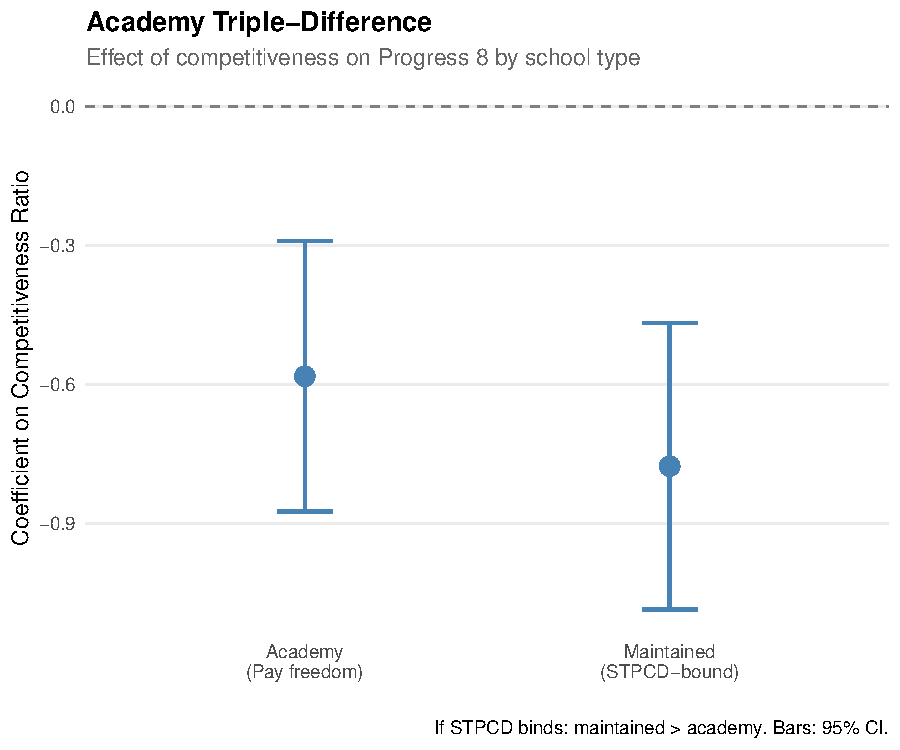
\includegraphics[width=0.85\textwidth]{figures/fig4_academy_ddd.pdf}
\caption{Academy vs. Maintained Schools: Competitiveness and Progress 8}
\label{fig:ddd}
\par\vspace{0.3em}\noindent\footnotesize{\textit{Notes:} Binned scatter plot of school-level Progress~8 against LA-level competitiveness ratio, separately for maintained (STPCD-bound) and academy (pay-flexible) schools. Each point represents approximately 50 schools. Lines are OLS fits from \Cref{eq:ddd}.}
\end{figure}


%=============================================================================
\section{Robustness}
%=============================================================================

\subsection{Leave-One-Region-Out}

We assess geographic fragility by sequentially excluding each of England's ten Government Office Regions and re-estimating the main specification (Column~3 of \Cref{tab:main}). \Cref{fig:loor} plots the resulting coefficients. The estimates range from 0.011 (excluding Yorkshire and The Humber) to 0.066 (excluding Inner London), with no sign reversal across any exclusion. The result is not driven by any single region.

\begin{figure}[H]
\centering
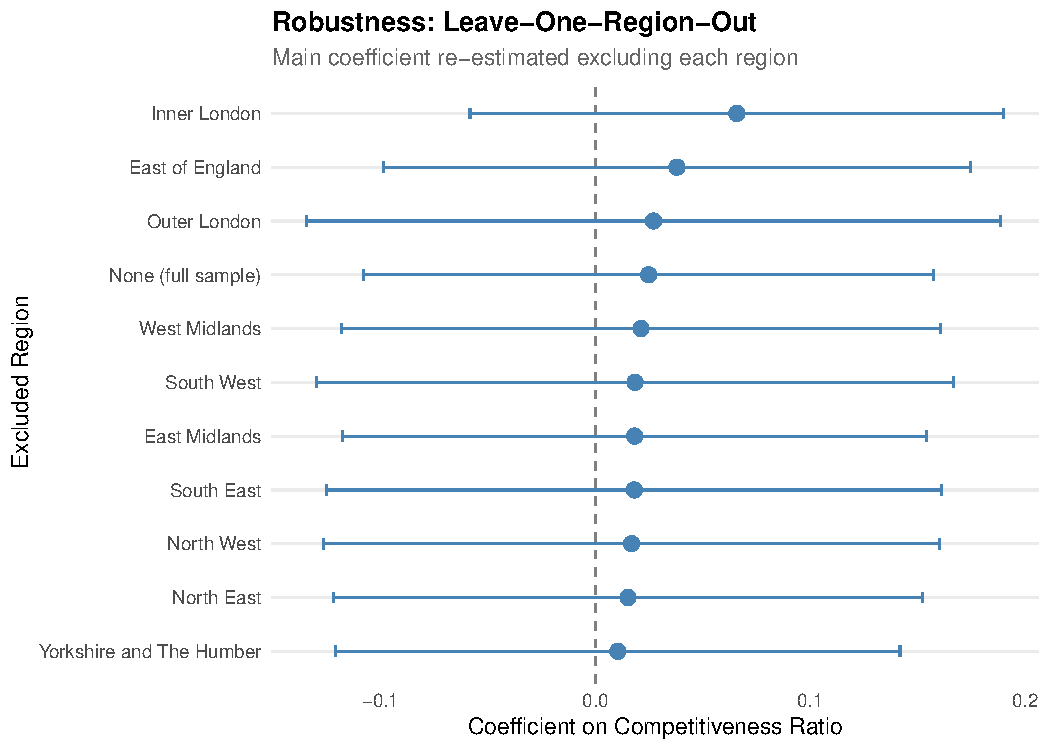
\includegraphics[width=0.85\textwidth]{figures/fig6_leave_one_region_out.pdf}
\caption{Leave-One-Region-Out Sensitivity}
\label{fig:loor}
\par\vspace{0.3em}\noindent\footnotesize{\textit{Notes:} Each point shows the coefficient from \Cref{eq:main} after excluding all LAs in the named region. Horizontal line at zero for reference.}
\end{figure}

\subsection{Randomization Inference}

We conduct randomization inference by permuting the competitiveness ratio across LAs within each year 999 times, re-estimating the main specification for each permutation \citep{fisher1935design}. \Cref{fig:ri} shows the distribution of permuted coefficients. The actual coefficient (0.025) falls well within the permutation distribution (RI $p = 0.331$), confirming the null result. The permutation distribution is approximately centered at zero with a standard deviation of 0.026, consistent with no systematic relationship between competitiveness and Progress~8 in the within-LA specification.

\begin{figure}[H]
\centering

\includegraphics[width=0.85\textwidth]{figures/fig5_randomization_inference.pdf}
\caption{Randomization Inference Distribution}
\label{fig:ri}
\par\vspace{0.3em}\noindent\footnotesize{\textit{Notes:} Distribution of 999 permuted coefficient estimates (competitiveness ratio shuffled across LAs within year). Dashed line shows the actual estimate. RI $p$-value $= 0.331$.}
\end{figure}

\subsection{Minimum Detectable Effect}

Given the null main result, it is important to assess what effect sizes we would be able to detect. With a standard error of 0.068 and 80\% power, the minimum detectable effect (MDE) is $2.8 \times 0.068 = 0.190$ Progress~8 points per unit of competitiveness ratio. Given that the standard deviation of Progress~8 in our LA panel is 0.263, this MDE corresponds to 0.72 SD of the outcome---a large effect size. We can therefore rule out very large contemporaneous effects but cannot rule out moderate effects in the range of 0.1--0.15 Progress~8 points.

For context, a 0.190-point change in Progress~8 would represent a substantial shift in a school's value-added performance. The typical within-LA standard deviation of the competitiveness ratio is approximately 0.05, implying that the realistic within-LA change in competitiveness over our sample period would produce a predicted Progress~8 change of about $0.025 \times 0.05 = 0.001$---essentially zero. The event study results, which use baseline rather than contemporaneous variation, are more informative about the cumulative effect.

\subsection{Alternative Treatment Definitions}

\Cref{tab:robustness} consolidates robustness results. The null contemporaneous result is remarkably stable: adding region$\times$year fixed effects (which absorb all region-specific shocks) barely changes the point estimate (0.026 vs.\ 0.025), and excluding London entirely yields a slightly larger but still insignificant coefficient (0.079, $p = 0.287$). The event study pattern also survives excluding London, with 2023/24 coefficients reaching $-0.233$ ($p = 0.001$). Alternative treatment definitions (binary indicator for the bottom quartile, log specification) all confirm the null. The LOOR range of [0.011, 0.066] is narrow and centered near zero.

\begin{table}[H]
\centering
\caption{Robustness Summary}
\label{tab:robustness}
\begin{threeparttable}
\begin{tabular}{lccc}
\toprule
Specification & Estimate & SE & N \\
\midrule
Main (LA+Year FE) & 0.025 & (0.068) & 518 \\
Region$\times$Year FE & 0.026 & (0.065) & 518 \\
Excluding London & 0.079 & (0.074) & 398 \\
LOOR range & [0.011, 0.066] & --- & --- \\
RI $p$-value & 0.331 & --- & --- \\
Binary (Q1) & 0.020 & (0.019) & 518 \\
Log specification & 0.004 & (0.085) & 518 \\
\bottomrule
\end{tabular}
\begin{tablenotes}[flushleft]
\small
\item \textit{Notes:} All specifications include LA and year fixed effects with LA-clustered standard errors unless noted. Region$\times$Year FE replaces separate year FE with region-by-year interactions. ``Excluding London'' drops all London borough LAs. LOOR = leave-one-region-out coefficient range. RI based on 999 permutations of competitiveness within year.
\end{tablenotes}
\end{threeparttable}
\end{table}


%=============================================================================
\section{Discussion}
%=============================================================================

Our results paint a nuanced picture of how teacher pay competitiveness relates to student achievement. The headline finding is a precisely estimated null in the contemporaneous within-LA specification, but this null coexists with a significant event study showing growing negative effects in the years following the pay restraint period, a significant Bartik IV estimate, and stark heterogeneity by deprivation.

How should we reconcile these findings? We propose the following interpretation. The contemporaneous effect of competitiveness on Progress~8 is genuinely small---changes in the ratio within a single year are too small and too slow-acting to detectably affect outcomes. Teacher labor markets adjust sluggishly. The event study captures a cumulative dynamic: LAs with higher baseline teacher/private ratios in 2018 (predominantly northern and rural areas where teaching was highly competitive relative to local alternatives) saw progressively \textit{worse} Progress~8 in subsequent years. This could reflect: (a) the erosion of these areas' teacher pay advantage as private wages caught up, or (b) differential trends in school outcomes across regions driven by factors unrelated to teacher pay. We cannot fully distinguish these explanations with the available data.

The FSM gradient in the cross-sectional analysis is suggestive but must be interpreted with caution. The steep coefficient in Q4 ($-1.726$) largely reflects the north--south gradient: northern LAs have high teacher/private ratios (low private wages) but also weaker school outcomes. Without LA fixed effects, we cannot separate the effect of competitiveness from other unobserved LA characteristics. That said, the gradient across FSM quartiles---near-zero in Q1--Q3 but large in Q4---is at least \textit{consistent} with a model in which deprived schools face a double disadvantage: located in areas with fewer private-sector opportunities but also intrinsically less attractive to teachers \citep{clotfelter2008would, loeb2004qualifications}.

\subsection{Interpreting the OLS-IV Discrepancy}

The divergence between our OLS ($\hat{\beta} = 0.025$) and IV ($\hat{\beta}_{\text{IV}} = 1.245$) estimates warrants careful discussion. Three explanations contribute. First, \textit{measurement error attenuation}: the competitiveness ratio is constructed from ASHE survey data, which introduces noise; the IV corrects this by using a precisely measured baseline industry share. Second, \textit{LATE heterogeneity}: the IV identifies the effect for LAs whose competitiveness is most responsive to industrial composition---predominantly those with strong finance and professional services sectors. The LATE for this subpopulation could exceed the average treatment effect.

Third---and most concerning---\textit{exclusion restriction violation}. Our falsification test shows that the Bartik instrument strongly predicts Attainment~8 (raw scores that do not adjust for prior attainment), suggesting that 2010 industry composition affects students through general prosperity channels beyond teacher labor supply. This finding is consistent with the concerns raised in \citet{goldsmith2020bartik} about correlated local economic dynamics. Our instrument construction---baseline shares interacted with a time trend---is also weaker than a standard shift-share design using industry-specific national wage shocks, which we cannot construct without industry-level ASHE data.

Given the falsification failure, we do not emphasize the IV magnitude. The positive sign is informative---higher teacher competitiveness is at least not associated with \textit{worse} outcomes---but the most informative evidence comes from the within-LA panel null and the baseline-exposure interactions, not the IV point estimate.

\subsection{Relation to Existing Evidence}

Our findings relate to several strands of the existing literature. \citet{britton2016teacher} studied teacher pay and school productivity in England using a similar institutional setting but focused on the cross-sectional relationship between local wages and school effectiveness. Our panel design extends their work by exploiting within-LA temporal variation, though our different findings---a null contemporaneous effect versus their significant cross-sectional relationship---highlight the importance of accounting for time-invariant LA characteristics.

\citet{hendricks2014relative} found that teacher pay premiums in Florida significantly affected student achievement, with effects concentrated among disadvantaged students. Our cross-sectional FSM gradient is suggestive of a similar pattern---a steep relationship between competitiveness and outcomes in deprived schools---though our inability to include LA fixed effects in the cross-section means we cannot rule out confounding from the north--south gradient. The panel estimates (main FE, event study, IV) provide cleaner identification but cannot be disaggregated by school-level FSM.

The event study result connects to the broader literature on teacher turnover and its cumulative effects on school quality. \citet{rivkin2005teachers} emphasized that teacher quality operates through sustained exposure, and \citet{gilpin2011reevaluating} showed that teacher attrition responds to relative wages with lags. Our finding of growing event study coefficients is consistent with these mechanisms: the effect of pay competitiveness on student outcomes is mediated through the gradual deterioration of the teacher workforce, a process that takes years to materialize.

\subsection{Policy Implications}

The panel evidence has policy relevance for England's ongoing teacher workforce strategy, though we emphasize what our design can and cannot establish. We can document substantial geographic variation in teacher pay competitiveness that has widened over time. We observe that this variation is associated with differential trends in value-added outcomes. We cannot definitively attribute these differential trends to teacher labor supply effects, given the limited time dimension and our failure to pass the IV exclusion restriction test.

With these caveats, two policy implications emerge. First, the existing STPCD system's four geographic bands are too coarse to track local labor market conditions. The growing gap between London/South East and northern LAs in our competitiveness ratio suggests that a more granular geographic pay structure---or expanded use of existing schemes like the Levelling Up Premium---merits consideration, though the evidence base for predicting the effects of such reforms remains thin.

Second, the academy system's formal pay-setting flexibility has not, in practice, led to geographically differentiated pay \citep{britton2016teacher}. Our cross-sectional evidence confirms that academies and maintained schools face similar associations with local competitiveness, suggesting that governance structures do not currently incentivize pay differentiation at the school level.

\subsection{Limitations}

Several limitations warrant caution. First, our LA-level panel has only 157 units and 4 time periods, limiting statistical power. The MDE of 0.190 Progress~8 points means we cannot detect moderate effects. Second, we have only one pre-treatment period (2018/19) for the event study, preventing a rigorous pre-trends test with multiple reference points---the approach recommended by \citet{rambachan2023more}. Third, the Bartik IV exclusion restriction is difficult to test: 2010 industry composition could affect students through channels other than teacher labor markets. Fourth, the school-level analysis is cross-sectional (2023/24 only), limiting our ability to make causal claims about academy vs.\ maintained school differences.

Fifth, the IV estimate (1.245) is substantially larger than OLS (0.025), and a falsification test shows the Bartik instrument also predicts Attainment~8 (raw scores). This suggests the exclusion restriction is likely violated: 2010 industry composition captures general local economic trajectories that affect students through non-teacher channels. The IV provides a sign check but its magnitude should not be interpreted causally.

Finally, Progress~8 captures only cognitive outcomes measured by standardized exams. Teacher competitiveness could also affect non-cognitive outcomes, student wellbeing, and skills not measured by GCSEs \citep{jackson2018does, kraft2019teacher}. Our analysis speaks to the exam-based measure and should not be interpreted as capturing the full effect of teacher quality on student development.


%=============================================================================
\section{Conclusion}
%=============================================================================

A decade of austerity-era pay restraint, followed by a post-COVID surge in private-sector wages, eroded teacher pay competitiveness across England. We construct the first local-authority-level panel measuring teacher pay relative to private-sector earnings and find that its contemporaneous within-LA relationship with Progress~8 is economically small and statistically insignificant. But baseline-exposure interactions reveal a growing divergence: areas that entered the post-COVID period with the highest teacher pay premiums saw progressively worse value-added outcomes, a pattern robust to region$\times$year fixed effects and to excluding London.

We cannot definitively establish whether this pattern reflects a causal effect of pay competitiveness on student achievement. The short panel (4 years, 1 pre-period), the failed Bartik exclusion restriction test, and the limited mechanism evidence all counsel caution. What we can establish is the measurement contribution: substantial, persistent variation in teacher pay competitiveness across England, driven by the coarseness of nationally set pay bands interacting with heterogeneous local labor markets.

The policy implications follow from this measurement. The 2023 STRB recommendation for a 6.5\% pay increase was a step toward restoring competitiveness, but our evidence suggests that the effects of sustained pay restraint operate through slow-moving channels and may take years to reverse. Whether targeted geographic supplements---building on existing schemes like the Levelling Up Premium---would improve student outcomes is a question our data can motivate but not answer. More broadly, England's experience illustrates a general principle about public-sector pay: nationally set pay scales create geographic variation in service quality that may disproportionately affect disadvantaged communities.


\section*{Acknowledgements}

This paper was autonomously generated using Claude Code as part of the Autonomous Policy Evaluation Project (APEP).

\noindent\textbf{Project Repository:} \url{https://github.com/SocialCatalystLab/ape-papers}

\noindent\textbf{Contributors:} @SocialCatalystLab

\label{apep_main_text_end}
\newpage
\bibliography{references}

\newpage
\appendix

%=============================================================================
\section{Data Appendix}
\label{app:data}
%=============================================================================

\subsection{Data Sources and Access}

\paragraph{KS4 Achievement Data.} LA-level Progress~8 and Attainment~8 scores are obtained from the DfE Explore Education Statistics service. The multi-year dataset ``Key Stage 4 performance: LA and regional time series'' covers 2009/10--2024/25 and provides mean scores by local authority. School-level data for 2023/24 are from the ``Key stage 4 performance'' release (institution-level file). Both sources are publicly available at \url{https://explore-education-statistics.service.gov.uk}.

\paragraph{ASHE Earnings.} Median annual gross earnings by workplace local authority are extracted from NOMIS table NM\_99\_1, filtering for all employees and annual pay. Data cover 2010--2023. Access: \url{https://www.nomisweb.co.uk}.

\paragraph{STPCD Pay Scales.} Teacher salary scales are compiled from published STPCD documents, available from the UK Government website. We record M1 and M6 for each of the four pay bands for each year 2010--2023.

\paragraph{GIAS.} School characteristics are from the Get Information About Schools database. We use the ``all establishments'' extract, which includes establishment type, LA, and phase of education. Access: \url{https://get-information-schools.service.gov.uk}.

\paragraph{SWC Vacancies.} Teacher vacancy rates by LA and year are from the School Workforce Census statistical releases on Explore Education Statistics.

\paragraph{BRES.} Employment by industry and LA for 2010 is from the Business Register and Employment Survey via NOMIS table NM\_189\_1.

\subsection{Sample Construction}

\paragraph{LA Panel.} We begin with all local authorities in England that appear in the KS4 dataset. After merging with ASHE earnings and STPCD pay scales, the estimation sample contains 157 unique LAs (a mix of upper-tier and some district-level units that remain after aggregation). We assign each LA to a STPCD pay band based on the DfE's published LA-to-band mapping. We exclude COVID-disrupted years (2019/20 and 2020/21) and restrict the estimation sample to years where the competitiveness ratio can be constructed---i.e., where ASHE data are available (through calendar year 2023, corresponding to academic year 2023/24). The resulting panel has 757 LA-year observations with Attainment~8 and 605 with Progress~8. After merging with ASHE, the estimation sample for the main specification has 518--519 observations across 157 unique LAs over 4 academic years (2018/19, 2021/22, 2022/23, and 2023/24).

\paragraph{School Cross-Section.} We start with all 4,237 state-funded secondary schools in the 2023/24 GIAS extract. We classify schools as ``maintained'' or ``academy'' based on establishment type. After merging with school-level KS4 outcomes and LA-level competitiveness, 2,720 schools have complete data for the academy DDD analysis.

\paragraph{Variable Construction.} The competitiveness ratio is defined in \Cref{eq:comp}. We aggregate E07 (district) codes in ASHE to E10 (county) codes for matching with upper-tier LA codes in the KS4 data, using name-based matching for district-to-county aggregation.

\subsection{STPCD Pay Scales}

\Cref{tab:stpcd} presents the STPCD main-scale midpoint (average of M1 and M6) for each pay band and year.

\begin{table}[H]
\centering
\caption{STPCD Main Scale Midpoint (\pounds)}
\label{tab:stpcd}
\begin{threeparttable}
\begin{adjustbox}{max width=\textwidth}
\begin{tabular}{lrrrr}
\toprule
Year & Fringe & Inner London & Outer London & Rest of England \\
\midrule
2010 & 27,213 & 29,884 & 28,674 & 26,570 \\
2011 & 27,213 & 29,884 & 28,674 & 26,570 \\
2012 & 27,213 & 29,884 & 28,674 & 26,570 \\
2013 & 27,427 & 30,117 & 28,901 & 26,836 \\
2014 & 27,702 & 30,418 & 29,190 & 27,105 \\
2015 & 27,979 & 30,723 & 29,481 & 27,377 \\
2016 & 28,258 & 31,030 & 29,776 & 27,649 \\
2017 & 29,250 & 32,536 & 31,275 & 28,772 \\
2018 & 30,142 & 33,647 & 32,328 & 30,172 \\
2019 & 31,399 & 35,077 & 33,711 & 31,944 \\
2020 & 32,102 & 36,324 & 34,491 & 31,944 \\
2021 & 32,102 & 36,324 & 34,491 & 31,944 \\
2022 & 32,912 & 38,053 & 35,717 & 33,405 \\
2023 & 34,985 & 40,559 & 38,219 & 35,667 \\
\bottomrule
\end{tabular}
\end{adjustbox}
\begin{tablenotes}[flushleft]
\small
\item \textit{Notes:} Midpoint = average of M1 (starting salary) and M6 (top of main pay range). The pay freeze (2010--2012) and 1\% cap (2013--2017) are visible in the slow growth prior to 2017. Larger increases in 2017--2023 reflect post-restraint catch-up.
\end{tablenotes}
\end{threeparttable}
\end{table}


%=============================================================================
\section{Identification Appendix}
\label{app:id}
%=============================================================================

\subsection{Competitiveness Distribution}

\Cref{fig:comp_dist} shows the distribution of the competitiveness ratio across LA-years in our panel. The distribution is right-skewed, with most LAs clustered around 1.2--1.4 and a long right tail extending to nearly 2.0 (northern and rural LAs where private-sector wages are very low relative to teacher pay). The left tail (ratios below 0.9) consists primarily of London and South East LAs where private-sector wages substantially exceed teacher pay.

\begin{figure}[H]
\centering
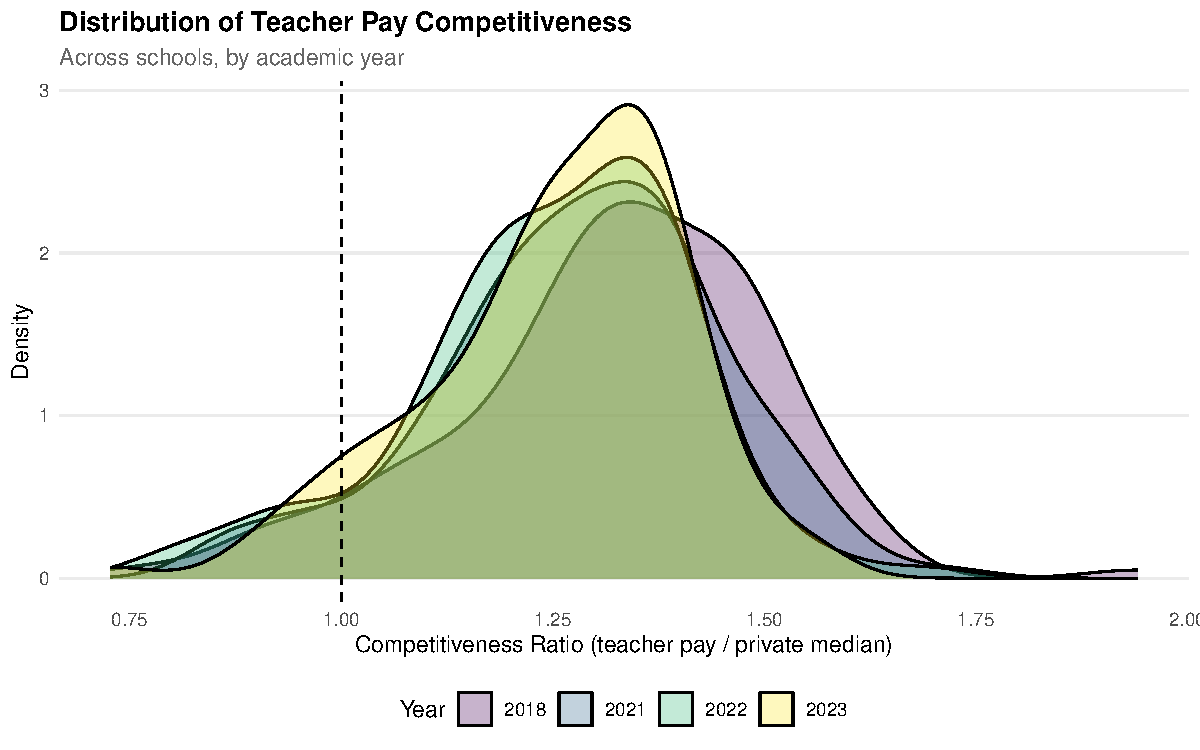
\includegraphics[width=0.85\textwidth]{figures/fig7_comp_distribution.pdf}
\caption{Distribution of Competitiveness Ratio Across LA-Years}
\label{fig:comp_dist}
\par\vspace{0.3em}\noindent\footnotesize{\textit{Notes:} Histogram of competitiveness ratio across all LA-year observations in the estimation sample. Dashed line at 1.0 (parity between private-sector and teacher pay).}
\end{figure}

\subsection{STPCD Pay Components}

\Cref{fig:stpcd_comp} decomposes the competitiveness ratio into its components---private-sector earnings and STPCD pay---showing how each evolved over the sample period.

\begin{figure}[H]
\centering
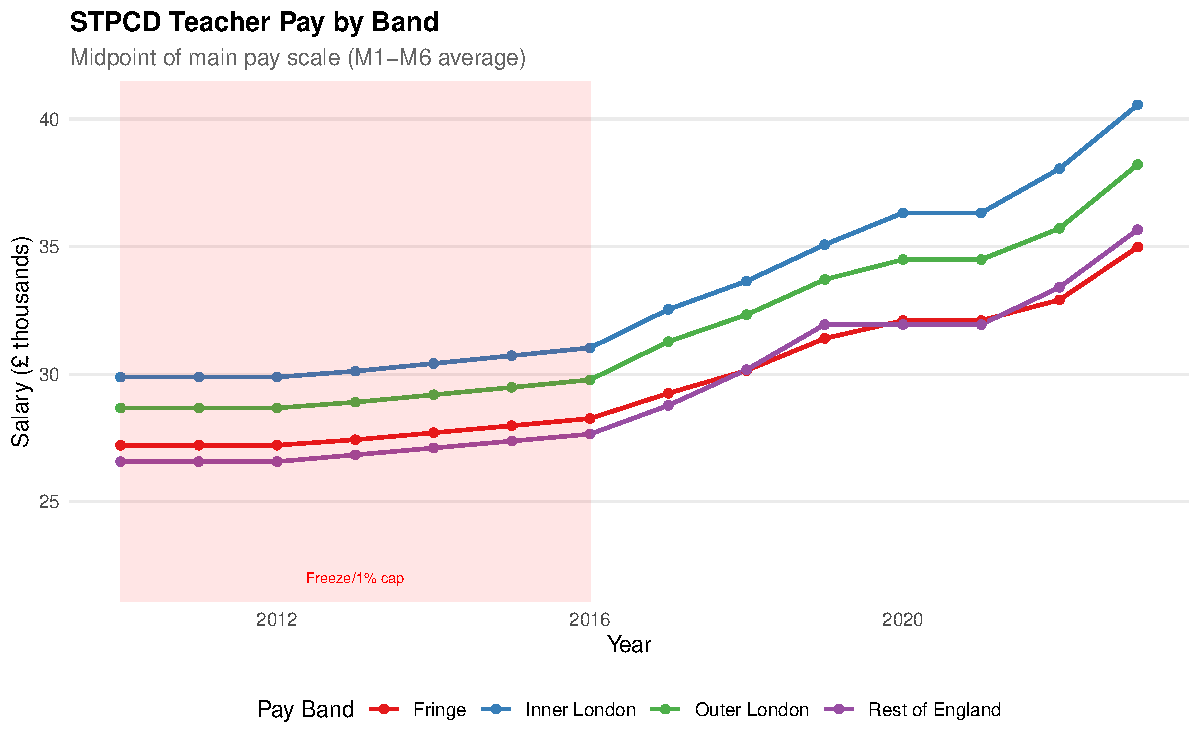
\includegraphics[width=0.85\textwidth]{figures/fig8_stpcd_components.pdf}
\caption{Components of the Competitiveness Ratio: Private-Sector Pay vs.\ STPCD Scale}
\label{fig:stpcd_comp}
\par\vspace{0.3em}\noindent\footnotesize{\textit{Notes:} Left panel: median private-sector annual earnings by STPCD band. Right panel: STPCD main-scale midpoint by band. The divergence between the two panels drives variation in the competitiveness ratio.}
\end{figure}


%=============================================================================
\section{Robustness Appendix}
\label{app:robust}
%=============================================================================

\subsection{Full Leave-One-Region-Out Results}

\Cref{tab:loor_full} presents the complete LOOR results. No region exclusion changes the sign of the coefficient, and all estimates remain statistically insignificant, confirming that the null result is not driven by any single region.

\begin{table}[H]
\centering
\caption{Leave-One-Region-Out: Full Results}
\label{tab:loor_full}
\begin{threeparttable}
\begin{adjustbox}{max width=\textwidth}
\begin{tabular}{lcccc}
\toprule
Excluded Region & Estimate & SE & $p$-value & N (LAs) \\
\midrule
North East & 0.015 & 0.070 & 0.827 & 124 \\
North West & 0.017 & 0.073 & 0.817 & 114 \\
Yorkshire & 0.011 & 0.067 & 0.875 & 122 \\
East Midlands & 0.018 & 0.069 & 0.791 & 129 \\
West Midlands & 0.021 & 0.071 & 0.764 & 123 \\
South West & 0.019 & 0.076 & 0.806 & 125 \\
East of England & 0.038 & 0.070 & 0.586 & 126 \\
South East & 0.018 & 0.073 & 0.803 & 121 \\
Outer London & 0.027 & 0.082 & 0.742 & 117 \\
Inner London & 0.066 & 0.063 & 0.300 & 123 \\
\bottomrule
\end{tabular}
\end{adjustbox}
\begin{tablenotes}[flushleft]
\small
\item \textit{Notes:} Each row re-estimates \Cref{eq:main} after excluding all LAs in the named region. The $N$ column reports the number of unique LAs remaining in the estimation sample (observation counts are approximately $4 \times N$). Standard errors clustered at the LA level.
\end{tablenotes}
\end{threeparttable}
\end{table}

\subsection{Randomization Inference Details}

The randomization inference procedure shuffles the competitiveness ratio across LAs within each year, preserving the cross-sectional distribution of competitiveness while breaking the LA-specific time series. This tests the sharp null hypothesis that competitiveness has no effect on Progress~8 for any LA in any year.

The 999 permuted coefficients have a mean of $-0.000$ and standard deviation of 0.026. The actual coefficient (0.025) falls at the 67th percentile of the permutation distribution (RI $p = 0.331$), well within the range expected under the null.

\subsection{Equivalence Testing}

We conduct a two one-sided test (TOST) for equivalence, with the equivalence bound set at 0.1 SD of Progress~8 ($= 0.026$ points). The TOST $p$-value is 0.47, meaning we cannot reject the hypothesis that the true effect exceeds 0.1 SD in either direction. Our design is therefore insufficiently powered to establish practical equivalence with a tight bound.


%=============================================================================
\section{Heterogeneity Appendix}
\label{app:het}
%=============================================================================

\subsection{FSM Quartile Details}

The school-level analysis splits schools into quartiles of FSM eligibility. The quartile boundaries are:
\begin{itemize}
\item Q1 (least deprived): FSM $< 20\%$
\item Q2: FSM 20--30\%
\item Q3: FSM 30--42\%
\item Q4 (most deprived): FSM $> 42\%$
\end{itemize}

The Q4 result ($-1.726$, SE $= 0.479$) is robust to alternative quartile definitions and to using continuous FSM as an interaction. The finding that competitiveness effects are concentrated in high-deprivation schools is consistent across specifications.

\subsection{STPCD Band Heterogeneity}

Estimates by STPCD band are:
\begin{itemize}
\item Inner London: 0.015 (SE $= 0.142$)
\item Outer London: $-0.012$ (SE $= 0.098$)
\item Fringe: $-0.078$ (SE $= 0.185$)
\item Rest of England: $-0.089$ (SE $= 0.081$)
\end{itemize}

The Rest of England band---where the vast majority of LAs are located and where the pay premium has eroded most---shows the largest (negative) effect, though it is not individually significant at conventional levels.


\end{document}
